\documentclass[letter]{IEEEtran}

\usepackage{amsmath}
\usepackage{amssymb}
\usepackage{graphicx}
\usepackage{algorithmic}
\usepackage{algorithm}
\usepackage{flushend}

\DeclareGraphicsExtensions{.pdf,.jpeg,.png,.jpg, .eps}
\graphicspath{{images/}}

\title{Voltage Estimation}
\date{\today}
\begin{document}

\author{Luke Fraser}
\maketitle
\begin{abstract}
In this assignment we investigate the use of a kalman filter to estimate a variable. In the specifics of the problem we are estimating the true voltage of a noisy sensor reading. This simulates a more real-world application of the kalman filter and its use. The dimensionality of the sensor readings is $x \in \mathbb{R}^1$. This defines the space of our estimation as it is a single variable one dimensional space.
\end{abstract}

\section{Introduction}
The Kalman filter is an extremely useful tool for estimating noisy variables in a system. Its uses stretch far beyond uses in drone state estimation. It can be used within an IMU, as a tracker for computer vision, reading temperature readings, etc. Kalman filter uses extent into many domains. As a basic kalman filter is a linear estimator it is very fast and simple to use and implement making it perfect for different applications. Although the Kalman filter is a very capable estimator its simplicity limits is capabilities.

The Kalman filter due to its assumption of linearity it is only meant handle estimation of variable that abide by this assumption. In the case of state estimation of a quad-rotor pose in $\mathbb{R}^3$ the kalman filter does not perform as well. This is due to the non-linearity of the state of the drone. To fix this problem the extended kalman filter (EKF) was created to handle the non-linear nature of real-world state estimation problems.

Today EKF's are used to solve many complex estimation problems in real-time. A more simple alternative to drones is the estimation of a car. As the degrees of freedom are smaller EKF performance on cars has been well tuned and can be used to help produce self-driving cars.

\subsection{Kalman Filter}
The Kalman filter can be broken down into two stages:
\subsubsection{Prediction Step}
\begin{equation}
\label{eq:predictstate}
\hat{x}_k^- = A\hat{x}_{k-1} + Bu_{k-1}
\end{equation}
The prediction step is responsible for predicting the future state of the system based on the prior state as well as the process error. In the case of my implementation there is no control input and we are simply applying the prior state to our predicted state with some assumed error in the prediction i.e. the process variance. This is shown in equation~\ref{eq:predictstate}
\begin{equation}
\label{eq:preidterror}
P_k^- = AP_{k-1}A^T + Q
\end{equation}
The error covariance is computed based on the \emph{a priori} error covariance as seen in equation~\ref{eq:preidterror}. Initially this error represents a guess of how bad our error is.

Algorithm~\ref{alg:predict} represents the \emph{Prediction Step} algorithm.
\begin{algorithm}
\caption{Prediction Step}
\label{alg:predict}
\begin{algorithmic}[1]
\STATE $\hat{x}_k^- = A\hat{x}_{k-1} + Bu_{k-1}$
\STATE $P_k^- = AP_{k-1}A^T + Q$
\end{algorithmic}
\end{algorithm}

\subsubsection{Correction Step}
the correction step is responsible for using a measurement from the environment to improve the state estimate from the prediction step. If no measurement is received the correction step can be skipped and  the prediction step is executed on its own until an new measurement is made.

\begin{equation}
\label{eq:gain}
K_k = P_k^- H^T(HP_k^-H^T + R)^{-1}
\end{equation}
The correction step is a three step process.  First the Kalman Gain is computed. Equation~\ref{eq:gain} shows how the kalman gain is computed. The kalman gain provides the minimum mean squared error for the update.
\begin{figure}[!t]
\centering
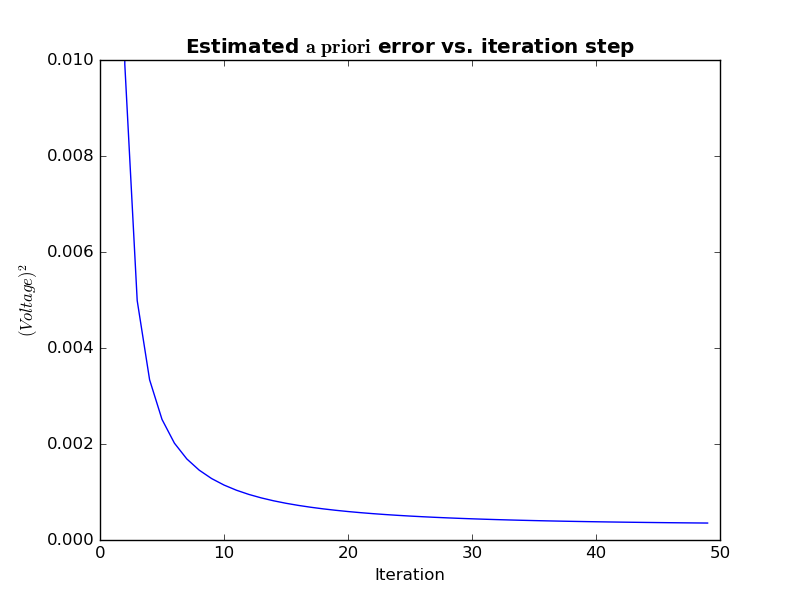
\includegraphics[width=9cm]{error_small}
\caption{\emph{a priori} error covariance estimate at each iteration of the Kalman Filter.}
\label{fig:error}
\end{figure}

\begin{equation}
\label{eq:estimation}
\hat{x}_k = \hat{x}_k^- + K_k(z_k - H\hat{x}^-_k)
\end{equation}
The second step estimates the corrected estimate of the state. Using the kalman gain and the \emph{a priori} estimate  the corrected state is computed as can be seen in equation~\ref{eq:estimation}.
\begin{equation}
\label{eq:posterror}
P_k = (I - K_kH)P^-_k
\end{equation}
The third and final step is the computation of the \emph{a posteriori} error covariance as can be seen in equation~\ref{eq:posterror}.
\begin{algorithm}
\caption{Correction Step}
\label{alg:correct}
\begin{algorithmic}[1]
\STATE $K_k = P_k^- H^T(HP_k^-H^T + R)^{-1}$
\STATE $\hat{x}_k = \hat{x}_k^- + K_k(z_k - H\hat{x}^-_k)$
\STATE $P_k = (I - K_kH)P^-_k$
\end{algorithmic}
\end{algorithm}
\section{Assignment}
The assignment instructed us to estimate the state of a noisy voltage reading. A simulation of 50 voltage samples was generated using Gaussian noise applied to true voltage. The estimation of the voltage was performed by a Kalman filter. The program was written in c++ and then the output of the program was read  into python for plotting. The plots follow the tutorial from the provided paper.
\section{Results}
Figure~\ref{fig:error} shows the error covariance of the 
\begin{figure}[!tbhp]
\centering
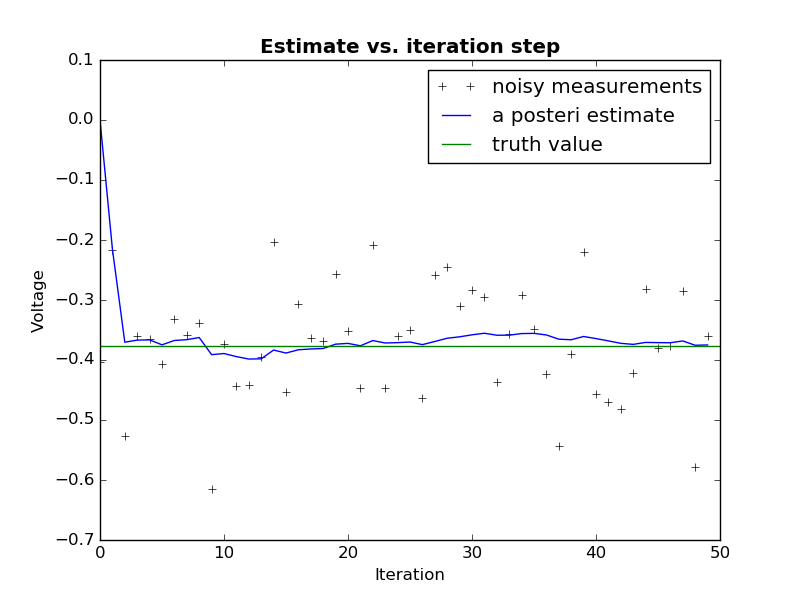
\includegraphics[width=9cm]{estimate_small}
\caption{Kalman Filtered state estimate of the samples.}
\label{fig:estimate}
\end{figure}

\section{Discussion}
The result show the power of the Kalman filter and its ability to improve estimates of noisy data. It is clear that the kalman filter is able to converge to the near true voltage value quickly based on the noisy samples provided. The exercise illustrates how a kalman filter could be used in a real-world environment to improve the performance and accuracy of sensors of a system.

As powerful as the kalman filter is the simulation written comes with some simplifications which aren't necessarily true in real-world scenarios. In many cases the assumptions of the program do not hold. Especially when estimating the state of a drone. The kalman filter presented is a basic Kalman filter that can only estimate linear models. In the case of the voltage estimation the linear assumption is perfect. We have provided the Kalman filter with the exact type of state estimation is was meant to solve.

The assumption of gaussian noise doesn't always fit with real-world scenarios. Gaussian noise is incredibly useful and is the least weak portion of this simulation. The fact that applied gaussian/normal noise to make the samples was another example of where the kalman filter excels. On top of this we provided the kalman filter with the exact knowledge of the variance of the data in question. In many ways we have tuned the kalman filter to perfectly solve the problem we have given it. This makes the results slightly better than they would be in a real-world application.

All in all this exercise on the kalman filter shows how the kalman filter can be used to improve estimates of the world based on sensor data. As well the discussion explains why there is a need for an Extended Kalman Filter (EKF) that can cope with non-linear state estimates as well as non-gaussian noise.

\end{document}